\section{Background}
This section provides a background on two main topics of the project: neural networks and machine translation. 

\subsection{Neural networks}
Neural networks are composed of highly interconnected processing units (or activation units) working together to approximate a function based on the input data. Nerual networks like feed-forward multi-layer perceptrons, shown in figure \ref{mlp}, can approximate any (continuous) function to an arbitrary accuracy if the number of hidden neurons are large enough \citep{hornik1989multilayer}. These networks can be trained using backpropogation algorithm \citep{rumelhart1988learning} by updating the weights and biases based on an objective function. As the training progresses, the networks updates its weights in a way that its predicted output moves closer to the original output. One layer feed-forward neural network can be written as follows


%of the network to match the predicted output to the labelled output
\begin{equation}
NN_{MLP1} (x) = g(xW^1 + b^1 )W^2 + b^2
\end{equation}

where g can be any non linear activation function, $x$ is an input vector, $W^1, W^2, b^1$ and  $b^2$ are the weights and biases for the network.

Unlike other machine learning approaches where input features have to be hand engineered, neural networks can learn the features required from the training data. 

\begin{figure}[ht]
	\centering
	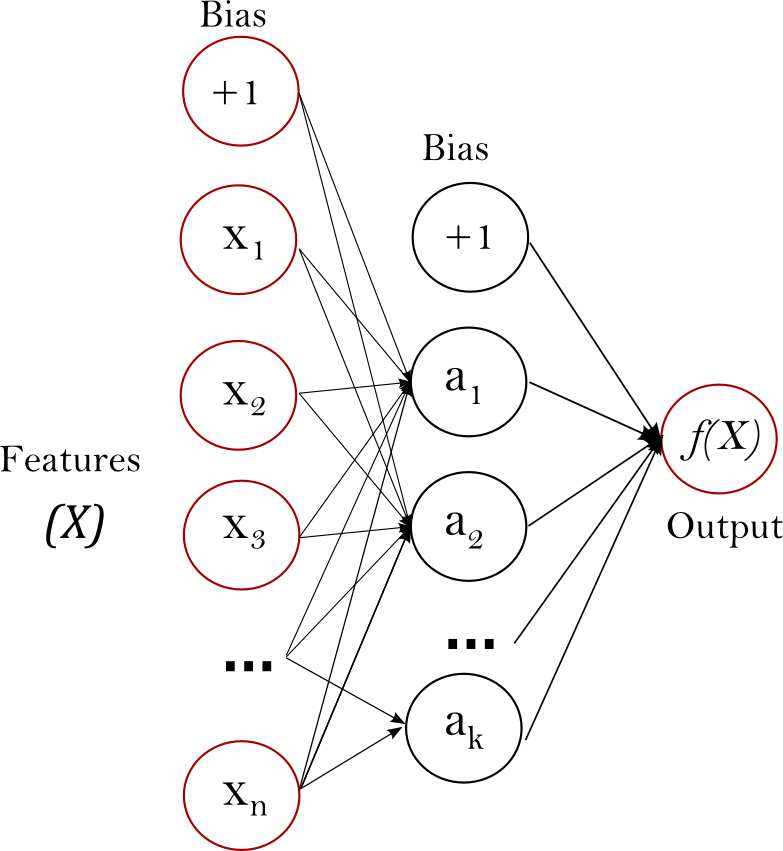
\includegraphics{images/multilayerperceptron_network}
	\caption{Multilayer perceptron network with one hidden layer \citep{pedregosa2011scikit}}
	\label{mlp}
\end{figure}

One class of neural network model called Recurrent Nerual Network (RNN) \citep{elman1990finding} is particularly well suited for machine translation. In natural languages, the input is sequence of words of arbitrary length based on some structure properties of the language. RNNs allow for representing an input sequence of arbitrary length as fixed-sized vectors based on its structural properties. A simple RNN \citep{goldberg2016primer} can be defined as follows.

\begin{align*}
h_{1:n},  y_{1:n} &= RNN(h_0,x_{1:n}) \\
h_i &= R(h_{i-1},x_i;\theta) \\
y_i &= O(h_i;\theta)
\end{align*}
\[ 
x_i \in \mathbb{R}^{d_{in}}, y_i \in \mathbb{R}^{d_{out}}, h_i \in \mathbb{R}^{f({d_{out}})} \]

where $x_{1:n}$ is the input vector, $y_{1:n}$ is the output vector and $h_{i}$ is the state vector at time-step $i$. $R$ is a non linear function applied over current input $x_i$ and previous hidden state $s_{i-1}$. $O$ is an additional function applied over current hidden state to generate output vector.  Parameters $\theta$ are shared across the network. A simple RNN uses $sigmoid$ or $tanh$ as the non linear function in the neural units. Special kind of neural units like Long Short-Term Memory (LSTM) \citep{hochreiter1997long} or Gated Recurrent Units (GRU) \citep{cho2014learning} can also be used. The same network is graphically represented in figure \ref{rnn}


\begin{figure}[ht]
	\centering
	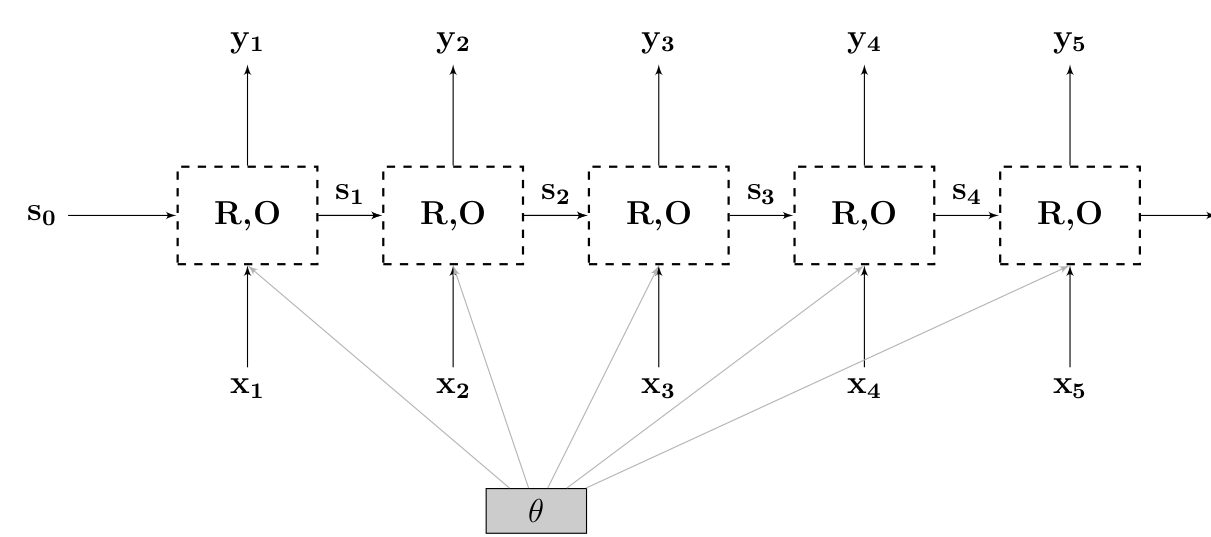
\includegraphics[scale=0.3]{images/rnn}
	\caption{Graphical representation of RNN \citep{goldberg2016primer}}.
	\label{rnn}
\end{figure}


It can be noticed that the input for these neural networks are a sequence of vectors not words. NMT systems use word embeddings to represent input words. It is a way of representing words in a vocabulary as vectors in a high dimensional space. These representations have been surprisingly good at capturing semantic and syntactic regularities in languages \citep{mikolov2013distributed}. When used as input, these models have also been shown to improve the performance of many NLP systems in tasks like MT \citep{vaswani2017attention, sennrich2015neural}, Sentiment Classification \citep{kumar2016ask}, part of speech tagging \citep{kumar2016ask}, etc., The vector representation for words in these models primarily depend on word co-occurrence or context words within a window size capturing syntactic, semantic and morphological properties of the words. 

%\begin{figure}[ht]
%	\centering
%	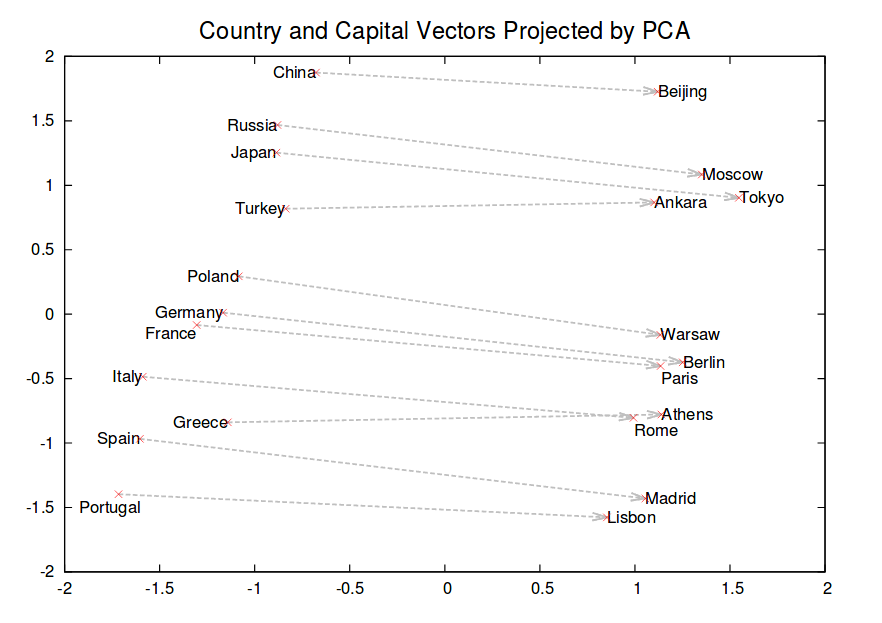
\includegraphics[scale=0.5]{images/embeddings}
%	\caption{Two-dimensional Principal component analysis (PCA) projection of 1000-dimensional vectors of countries and their capitals \citep{mikolov2013distributed}}.
%	\label{embeddings}
%\end{figure}


%\footnote{Principal component analysis (PCA is dimensionality technique used here to show high dimensional vectors in 2-dimensional space.)}

One of the major challenges for many embedding models is their inability to handle out of vocabulary words.  This problem is more pronounced in languages with rich morphology. A word in morphologically rich languages encodes more information (such as gender, number, tense) as compared to morphologically poor languages which rely on word order and context. Recently, many models have been proposed to solve this problem. \cite{sun2016inside} proposed a method to integrate both external contexts and internal morphemes to learn better word embeddings especially for rare and unknown words. \cite{bojanowski2016enriching} incorporate subword information like character n-grams\footnote{a character n-gram is a sequence of n characters from a word} for learning word embeddings during training. Overall, character embeddings models, where vector representations for every character or character n-grams are learned, have be shown to generate good word embeddings for rare and unknown words. 

%%Most of these models were originally developed in English - a language with strict word order and relatively poor morphology. These models perform the best in English. 
%

%
%
%Despite their advantages, NMT systems are not capable of translating rare and unknown words. In this project, I am implementing an end to end encoder-decoder system for machine translation and an unsupervised method to handle unknown and rare words.
%

\subsection{Machine Translation}
Machine translation is a task of translating a source language sentence $F$ to the target language sentence $E$ using computing resources. It can effectively remove human language barrier allowing assimilation of content from different languages.The potential of mt has led to substantial amount of research being done on the subject since the advent of digital computing. There have been many approaches to the problem like rule-based MT, phrase-based MT, NMT, etc. In the early days, rule based approaches that used dictionaries, grammar and pre-defined rules to translate text were explored until the ALPAC report in 1966. The ALPAC report showed that post-editing machine translation was not cheaper or faster than human translation. 

\subsubsection{Statistical Machine Translation}

In the late 1980s, following the success of statistical method on speech recognition, IBM research \citep{brown1993mathematics} modelled the problem of translation as a statistical optimization problem. Many SMT approaches like word-based models \citep{brown1993mathematics}, phrase-based models \citep{koehn2003statistical,marcu2002phrase}, hierarchical phrase-based  models \citep{chiang2007hierarchical} and syntax based models \cite{galley2004s,galley2006scalable} were proposed. The goal of these SMT systems is to maximize the probability of target sentence $f$ given the source language sentence $e$

\[ \underset{f}{argmax \  } P(f|e) = \underset{f}{arg max } (P(f) \times P(e|f)) \]

where $P(e)$ is a language model and $P(e|f)$ is a translation model. Language models learns to assign probability to a sequence of words in a language. They assign higher probability to sentences that are more likely to occur in the language and hence a measure of fluency in the the language. Language modelling is central many tasks in NLP including MT.  

Translation models learns the mapping between source and target language words or phrases. They measure word level translation accuracy between source and target sentence. These models were built by analyzing  monolingual, bilingual corpus and learning their probability distribution. The rise of digital text resources like parallel corpora and increase in computing power and storage fuelled the growth of SMT systems. Although SMT systems were robust to noisy data,  they required fine tuning for many components like language model, reordering model and translation model for each language pairs. They also require large amount of data and do not handle long range dependencies well.


\subsubsection{Neural Machine Translation}

NMT system is a neural network that models the conditional probability $p(y|x)$ of generating a target language $y$ sentence given the source language sentence $x$. Generally, any NMT systems consists of two components i) an \textit{encoder} that computes a sentence representation vector from the source sentence and ii) a \textit{decoder} that transforms the vector representation to a target language sentence. RNNs are a common choice of network for both encoders and decoder as they process input in a sequential fashion. Convolution neural networks have also been used especially as an encoder.

%In 2003, \cite{bengio2003neural} proposed probabilistic language model based on neural networks which laid the foundation for the use of neural networks in machine translation. 

Initially, neural networks were used as a component in phrase based systems to score the quality of translation \citep{schwenk2012continuous} or provide additional features to SMT systems \citep{zou2013bilingual}. \cite{kalchbrenner2013recurrent} proposed the first end to end approach for NMT using convolution neural networks as encoder and RNN as the decoder. Their network suffered from the problem of vanishing gradients where the network was unable to capture long range dependencies. To overcome this problem, a more sophisticated activation function like LSTM \citep{hochreiter1997long} or GRU \citep{cho2014learning} are used.  \cite{sutskever2014sequence} and \cite{cho2014learning} demonstrated that these gated units were able to handle long range dependencies better than simple RNN \citep{elman1990finding}. A encoder-decoder network with LSTM RNNs \citep{sutskever2014sequence} is shown in figure \ref{seq2seq}

\begin{figure}[ht]
	\centering
	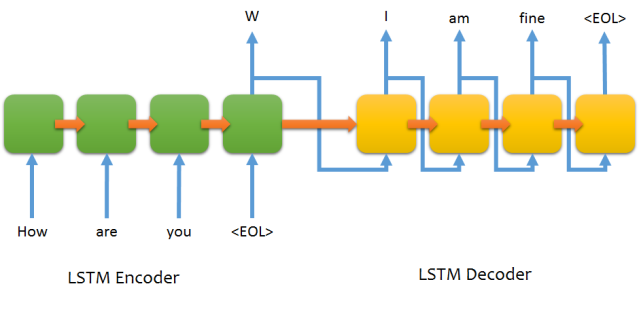
\includegraphics[scale=0.9]{images/seq2seq}
	\caption{RNN with LSTM encoder and decoder \citep{sutskever2014sequence}}.
	\label{seq2seq}
\end{figure}


These simple encoder-decoder networks summarize the source sentence in a fixed length context vector. \cite{bahdanau2014neural} noted that these networks were inadequate to represent long sentences due to the fixed dimension of the context vector. While this problem could theoretically be solved by increasing the dimension of the context vector, the limited computing power and memory sets an upper limit. \cite{bahdanau2014neural} proposed an attention based encoder-decoder architecture to mitigate this problem. In their additive approach, a single feed forward neural networks that can learn to assign different weights to the hidden layer vectors was used. The weighted sum of the hidden layer vectors called context vectors were calculated during each word prediction and used.  For this project, I will be implementing the attention based encoder-decoder model proposed in \cite{bahdanau2014neural} as base NMT system.


% Basics needed to understand the rest of the text with references to authoritative literature sources

%
%
%
%
%In their model, the source language sentence will be encoded into a real valued vector using the encoder. The decoder will decode the vector to a target language sentence to produce the output. 
%
%Unlike, SMT systems, NMT systems generalize well, do not require domain knowledge and are more tolerant to noisy data \cite{bibid}. 
%
%
%NMT systems use vector representation, also called word embeddings, for input words and internal states. Word embedding is a way of representing words in the vocabulary using vectors in a high dimensional space.Word embedding models like \cite{bengio2003neural,mikolov2013distributed,pennington2014glove} etc., learn word representation in continuous vector space where similar words are expected to occur closer to each other. These models have been successfully used in many NLP tasks like Machine Translation. The vector representation for word in most of these models primarily depend on word co-occurrence or context words within a window size capturing syntactic, semantic and morphological properties of natural languages. 
%
%
%%Most of these models were originally developed in English - a language with strict word order and relatively poor morphology. These models perform the best in English. 
%
%One of the major challenges for many embedding models is their inability to handle out of vocabulary words.  This problem is more pronounced in languages with rich morphology. A word in morphologically rich languages encodes more information (such as gender, number, tense) as compared to morphologically poor languages which rely on word order and context. 
%
%
%Despite their advantages, NMT systems are not capable of translating rare and unknown words. In this project, I am implementing an end to end encoder-decoder system for machine translation and an unsupervised method to handle unknown and rare words.
%






%In 2003, \cite{bengio2003neural} proposed a language model developed using neural network.
%
%Data Sparcity Problem.
